\begin{tikzpicture}
\node[anchor=south west,inner sep=0] at (0,0) {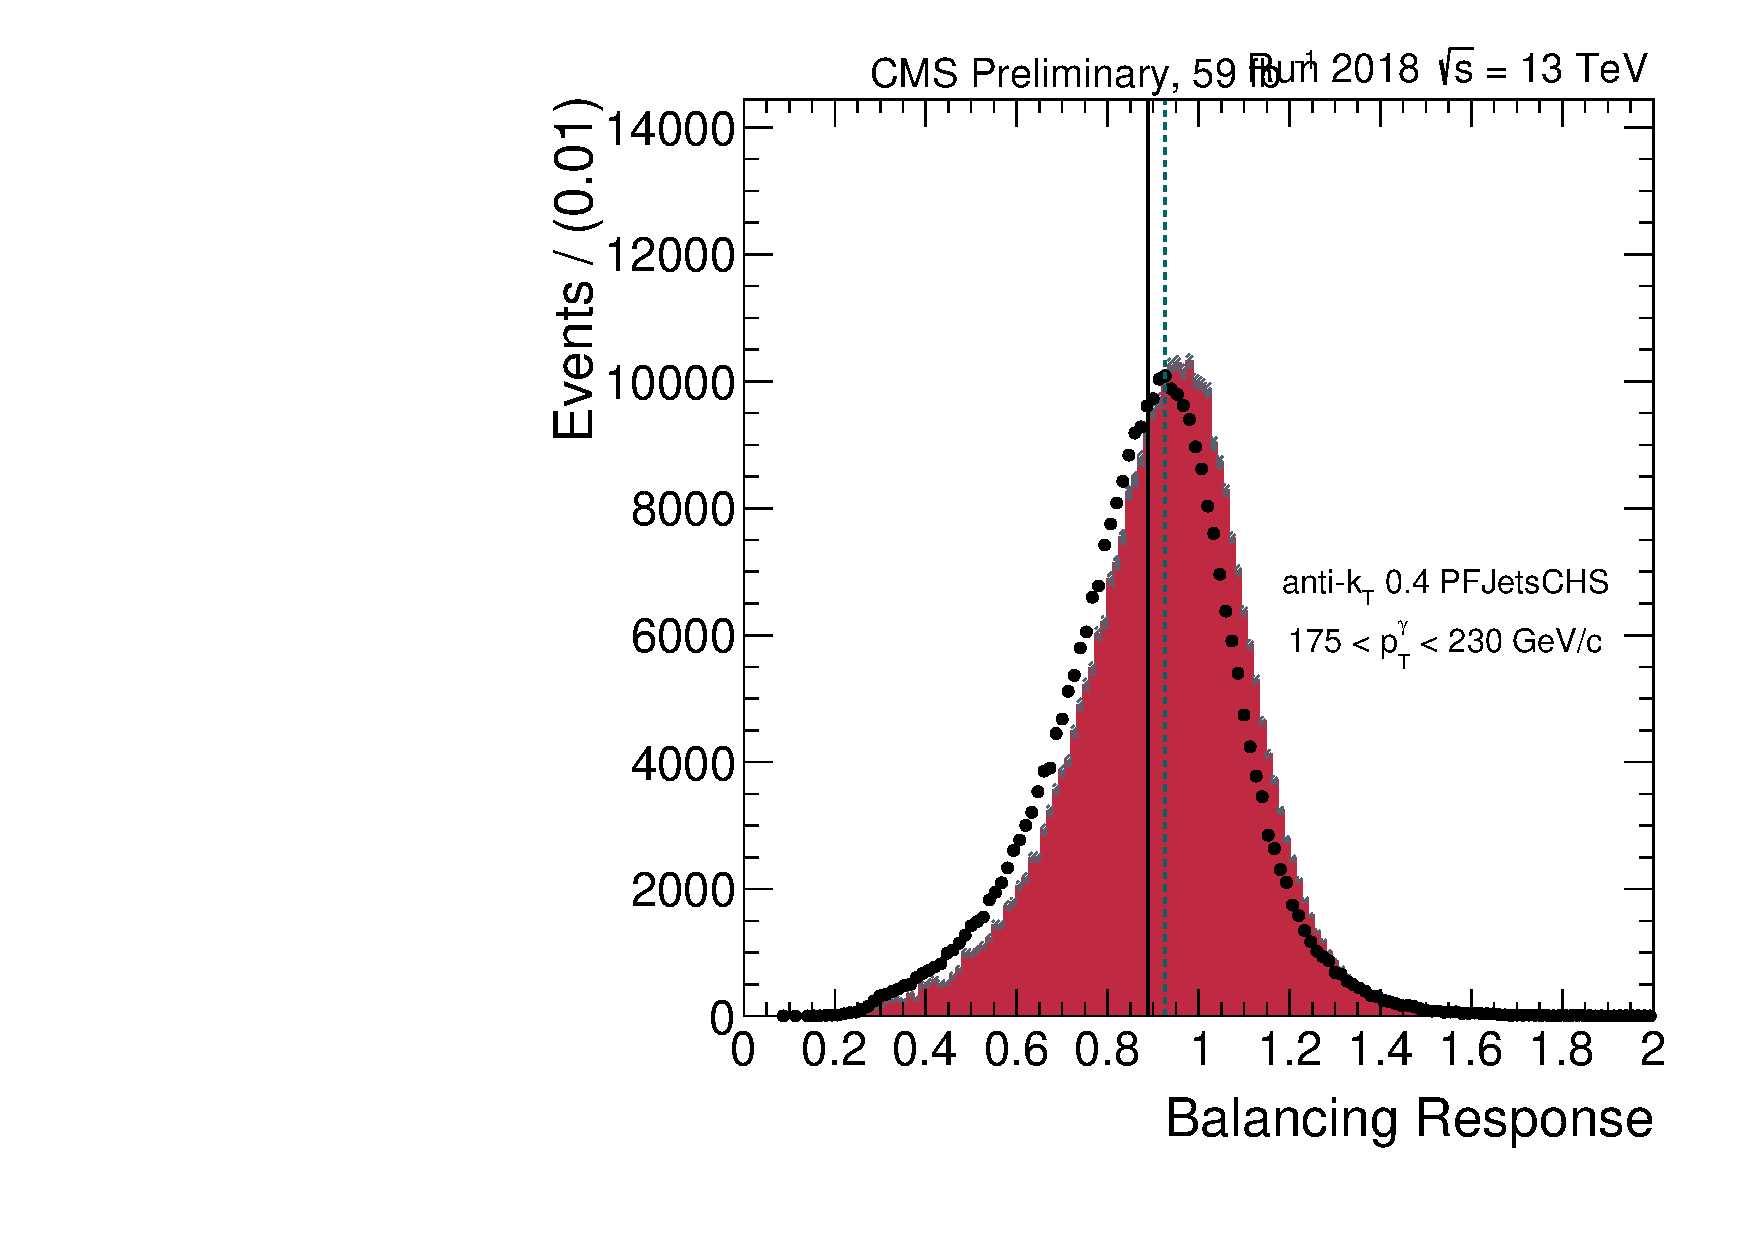
\includegraphics[width=8cm]{\PhDthesisdir/contents/chapter-JERC/JES/my_plots/distributions/2017UL/source/resp_balancing_eta0013_ptPhot_175_230.pdf}};

% above txt
\fill [white] (1.2, 7.4) rectangle (7.6,7.8);
\draw (7.6, 7.6) node [left] {\footnotesize \todo{\tiny DE plots placeholders} Run 2017 BCDEF, \SI{42}{\femto\barn^{-1}} (\SI{13}{\TeV})};

% masks
\fill [white] (0, 0) rectangle (8,1.1);
\fill [white] (0, 0) rectangle (1.4,7.4);

% X axis
\foreach \val in {0, 0.2, 0.4, 0.6, 0.8, 1, 1.2, 1.4, 1.6, 1.8, 2}{
\draw ({1.45+(7.51-1.45)*(\val)/(2)}, .95) node {\tiny $\num{\val}$};
}
\draw (7.5, .5) node [left] {\scriptsize \Rbal};

% Y axis
\foreach \val in {0, 500, ..., 4000}{
\draw (1.5, {1.15+\val/4000*(7.12-1.15)}) node [left] {\tiny $\num{\val}$};
}
\draw (.25, 7.25) node [left, rotate=90] {\scriptsize Nombre d'événements / \num{0.01}};

\end{tikzpicture}
